\documentclass[10pt]{beamer}

\usetheme[progressbar=frametitle]{metropolis}
\usepackage{appendixnumberbeamer}

\usepackage{booktabs}
\usepackage{svg}
\usepackage[scale=2]{ccicons}

\usepackage{pgfplots}
\usepgfplotslibrary{dateplot}

\usepackage{xspace}
\newcommand{\themename}{\textbf{\textsc{metropolis}}\xspace}
\usetikzlibrary{positioning}

\title{Finite Statemachines}
\subtitle{Specify and Implement dynamic Behaviour}
\date{\today}
\author{Stefan Dennig}
\institute{NewTec GmbH}
% \titlegraphic{\hfill\includegraphics[height=1.5cm]{logo.pdf}}

\begin{document}
\metroset{block=fill}
\maketitle

\section[Example]{Example}

\begin{frame}[fragile]{Example Button Debounce}
  \begin{columns}[T,onlytextwidth]
    \column{0.5\textwidth}
    Button Debounce Statemachine
    \begin{itemize}
      \item Button Inactive - Button is registered as released
      \item Button pressed - latch event after first pressed
      \item Button active - Button is registered as pressed
      \item Button released - latch event after first release
    \end{itemize}
    \column{0.5\textwidth}
      \begin{center}
        \includegraphics[keepaspectratio,scale=0.35]{out/buttonStatemachine.png}
      \end{center}
  \end{columns}
\end{frame}

\section[Theory]{Finite Statemachine}

\begin{frame}[fragile]{Definition}
  \begin{block}{Definition of a Statemachine}
    A finite-state machine (FSM) is a mathematical model of computation. 
    It is an abstract machine that can be in exactly one of a finite number of states at any given time. 
    The FSM can change from one state to another in response to some inputs; 
    the change from one state to another is called a transition.
  \end{block}
\end{frame}

\begin{frame}[fragile]{Definition}
  \begin{columns}[T,onlytextwidth]
    \column{0.5\textwidth}
      Parameters of a Statemachine:
      \begin{itemize}
        \item states $s$
        \item transitions $t$
        \item event $\sigma$
      \end{itemize}
      \begin{center}
      \begin{equation*}
        s \in \bold{S}
      \end{equation*}
    \end{center}
    \column{0.5\textwidth}
        \begin{block}{Definition of State}
          The state of a system is defined by the smallest possible number of its changeable internal parameters.
          e.g.: 
          \begin{itemize}
            \item velocity
            \item position
            \item temperature
          \end{itemize}
        \end{block}
    \end{columns}
\end{frame}

\begin{frame}[fragile]{Definition}
  \begin{columns}[T,onlytextwidth]
    \column{0.5\textwidth}
      Parameters of a Statemachine:
      \begin{itemize}
        \item states $s$
        \item transitions $t$
        \item event $\sigma$
      \end{itemize}
      \begin{center}
      \begin{equation*}
        t \in \bold{T}
      \end{equation*}
      \end{center}

    \column{0.5\textwidth}
        \begin{block}{Definition of Transition}
          A Transition is a change from one set of paramaters of a system to another one. 
          e.g.: 
          \begin{itemize}
            \item acceleration
            \item heat
          \end{itemize}
        \end{block}
    \end{columns}
\end{frame}

\begin{frame}[fragile]{Definition}
  \begin{columns}[T,onlytextwidth]
    \column{0.5\textwidth}
      Parameters of a Statemachine:
      \begin{itemize}
        \item states $s$
        \item transitions $t$
        \item event $\sigma$
      \end{itemize}
      \begin{center}
      \begin{equation*}
        \sigma \in \bold{\Sigma}
      \end{equation*}
      \end{center}

    \column{0.5\textwidth}
        \begin{block}{Definition of Event}
          A Event is a change of inputs of a system.
          e.g.: 
          \begin{itemize}
            \item push of gas pedal
            \item expiration of time
          \end{itemize}
        \end{block}
    \end{columns}
\end{frame}

\begin{frame}[fragile]{Definition}
  \begin{block}{Finite}
    A finite Statemachine only implements a limited set of states $\bold{S}$. This implicates a limited set of transitions $\bold{T}$ and a limited set of Events $\bold{E}$
  \end{block}

  A Statemachine can be described as a set functions $t$ operating on its internal state $s$. The output $y$ depends on the internal state $s$, additionaly it may depend on the input $\sigma$.
  \begin{center}
  \begin{equation}
    s_{n+1} = t(s_n,\sigma)
  \end{equation}
  \begin{equation}
    \lambda = g(s_n,\sigma)
  \end{equation}
  \end{center}
\end{frame}

\begin{frame}[fragile]{Mealy Machine}
  \begin{center}
      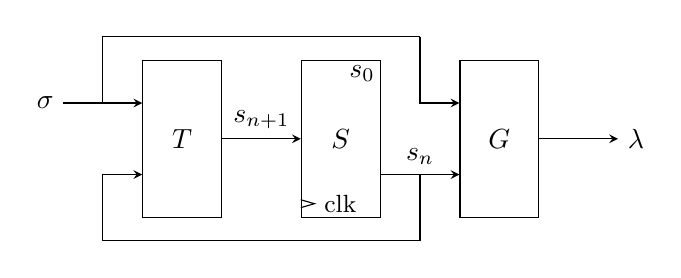
\begin{tikzpicture}
      \node [draw, minimum width=1cm, minimum height=2cm]  (input_logic) {$\bold{T}$};
      \node [draw, minimum width=1cm, minimum height=2cm, right=1cm of input_logic]  (memory) {$\bold{S}$};
      \node [draw, minimum width=1cm, minimum height=2cm, right=1cm of memory]  (output_logic) {$\bold{G}$};
      \node [below=0.33cm of input_logic.west]  (input_logic_state_in) {};
      \node [above=0.33cm of input_logic.west]  (input_logic_in_in) {};
      \node [above=0.33cm of output_logic.west]  (output_logic_in_in) {};
      \node [below=0.33cm of output_logic.west]  (output_logic_state_in) {};
      \node [below=0.33cm of memory.east]  (state_out) {};

      \draw [-stealth] (input_logic.east) -- (memory.west) node[midway,above]{$s_{n+1}$};
      \draw [-stealth] (state_out.center) -- (output_logic_state_in.center) node[midway] (state) {} node[midway,above] {$s_{n}$};
      \draw [stealth-] (input_logic_in_in.center) -- ++(-1,0) node[midway] (helper1) {} node[behind path, left]{$\sigma$};
      \draw [-stealth] (output_logic.east) -- ++(1,0) node[behind path, right]{$\lambda$};

      \node [below=1.5cm of helper1]  (helper2) {};
      \node [above=1.5cm of state]  (helper3) {};
      
      \draw (state.center) |- (helper2.center);
      \draw [-stealth] (helper2.center) |- (input_logic_state_in.center);
      \draw (helper1.center) |- (helper3.center);
      \draw [-stealth] (helper3.center) |- (output_logic_in_in.center);

  \node [below=0.75cm of memory.west]  (tri_a) {};
  \node [below=0.70cm of memory.west]  (tri_b_) {};
  \node [right=0.05cm of tri_b_.center]  (tri_b) {};
  \node [right=0.00cm of tri_b.center] (clock) {{\small clk}};
  \node [below=0.65cm of memory.west]  (tri_c) {};
  \draw (tri_a.center) -- (tri_b.center)  -- (tri_c.center);

  \node [below=0.05cm of memory.north east]  (s0_) {};
  \node [left=-0.05cm of s0_.center]  (s0) {$s_0$};

    \end{tikzpicture}

  \end{center}
  \begin{center}
  \begin{equation}
    s_{n+1} = t(s_n,\sigma)
  \end{equation}
  \begin{equation}
    \lambda = g(s_n,\sigma)
  \end{equation}
  \end{center}
\end{frame}

\begin{frame}[fragile]{Moore Machine}

\begin{center}
  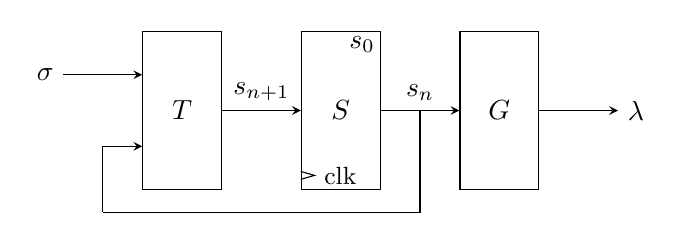
\begin{tikzpicture}

  \node [draw, minimum width=1cm, minimum height=2cm]  (input_logic) {$\bold{T}$};
  \node [draw, minimum width=1cm, minimum height=2cm, right=1cm of input_logic]  (memory) {$\bold{S}$};
  \node [draw, minimum width=1cm, minimum height=2cm, right=1cm of memory]  (output_logic) {$\bold{G}$};
  \node [below=0.33cm of input_logic.west]  (input_logic_state_in) {};
  \node [above=0.33cm of input_logic.west]  (input_logic_in_in) {};

  \draw [-stealth] (input_logic.east) -- (memory.west) node[midway,above]{$s_{n+1}$};
  \draw [-stealth] (memory.east) -- (output_logic.west) node[midway] (state) {} node[midway,above] {$s_{n}$};
  \draw [stealth-] (input_logic_in_in.center) -- ++(-1,0) node[midway] (helper1) {} node[behind path, left]{$\sigma$};
  \draw [-stealth] (output_logic.east) -- ++(1,0) node[behind path, right]{$\lambda$};

  \node [below=1.5cm of helper1]  (helper2) {};
  
  \draw (state.center) |- (helper2.center);
  \draw [-stealth] (helper2.center) |- (input_logic_state_in.center);

  \node [below=0.75cm of memory.west]  (tri_a) {};
  \node [below=0.70cm of memory.west]  (tri_b_) {};
  \node [right=0.05cm of tri_b_.center]  (tri_b) {};
  \node [right=0.00cm of tri_b.center] (clock) {{\small clk}};
  \node [below=0.65cm of memory.west]  (tri_c) {};
  \draw (tri_a.center) -- (tri_b.center)  -- (tri_c.center);

  \node [below=0.05cm of memory.north east]  (s0_) {};
  \node [left=-0.05cm of s0_.center]  (s0) {$s_0$};

  \end{tikzpicture}
\end{center}
  \begin{center}
  \begin{equation}
    s_{n+1} = t(s_n,\sigma)
  \end{equation}
  \begin{equation}
    \lambda = g(s_n)
  \end{equation}
  \end{center}
\end{frame}

\begin{frame}[fragile]{Medvedev Machine} 

\begin{center}
  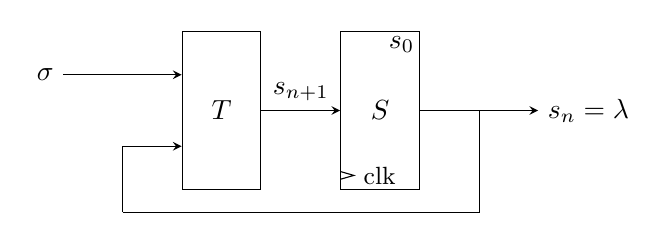
\begin{tikzpicture}

  \node [draw, minimum width=1cm, minimum height=2cm]  (input_logic) {$\bold{T}$};
  \node [draw, minimum width=1cm, minimum height=2cm, right=1cm of input_logic]  (memory) {$\bold{S}$};
  \node [below=0.33cm of input_logic.west]  (input_logic_state_in) {};
  \node [above=0.33cm of input_logic.west]  (input_logic_in_in) {};

  \draw [-stealth] (input_logic.east) -- (memory.west) node[midway,above]{$s_{n+1}$};
  \draw [-stealth] (memory.east) -- ++(1.5,0) node[midway] (state) {} node[behind path, right] {$s_{n} = \lambda$};
  \draw [stealth-] (input_logic_in_in.center) -- ++(-1.5,0) node[midway] (helper1) {} node[behind path, left]{$\sigma$};

  \node [below=1.5cm of helper1]  (helper2) {};
  
  \draw (state.center) |- (helper2.center);
  \draw [-stealth] (helper2.center) |- (input_logic_state_in.center);

  \node [below=0.75cm of memory.west]  (tri_a) {};
  \node [below=0.70cm of memory.west]  (tri_b_) {};
  \node [right=0.05cm of tri_b_.center]  (tri_b) {};
  \node [right=0.00cm of tri_b.center] (clock) {{\small clk}};
  \node [below=0.65cm of memory.west]  (tri_c) {};
  \draw (tri_a.center) -- (tri_b.center)  -- (tri_c.center);

  \node [below=0.05cm of memory.north east]  (s0_) {};
  \node [left=-0.05cm of s0_.center]  (s0) {$s_0$};

  \end{tikzpicture}

\end{center}
  \begin{center}
  \begin{equation}
    s_{n+1} = t(s_n,\sigma)
  \end{equation}
  \begin{equation}
    \lambda = s_n
  \end{equation}
  \end{center}
\end{frame}

\begin{frame}[fragile]{Facts}
 \begin{itemize}
  \item Statemachines, as per Definition, do not imply any timing behaviour.
  \item Every Memory implicitly holds state, thus implements a statemachine.
  \item The amount of states is proportional to the complexity of the statemachine.
  \item Every slightly complex component implements a statemachine.
  \item There can be multiple statemachines in a system.
 \end{itemize}
\end{frame}

\begin{frame}[fragile]{Design of Statemachines}
When to use a statemachine?
 \begin{itemize}
  \item Simple Behaviour that can be clustered
  \item Strict Deterministic control
  \item Ressource/Device Control
 \end{itemize}
When not to use a statemachine?
 \begin{itemize}
  \item If a combinational logic is an alternative
  \item If a mathematical formula can be used instead (filters)
  \item Multiple Statemachines should never implement the same state
 \end{itemize}
  \begin{alertblock}{Senior Experience}
    State should be avoided.
  \end{alertblock}
\end{frame}

\begin{frame}[fragile]{Designtips}
 \begin{itemize} 
  \item Decide about timing (cyclic, synchronous, asynchronous)
  \item Number of states shall be reduced
  \item Hierarchical Statemachines are a good way to reduce states
  \item Statemachines that are directly or indirectly linked shall be avoided
  \item Make states explicit (no rotation direction as variable, no global variables)
  \item If a component implies state implement it as a statemachine (init, running, error)
  \item shall invalid transitions be neglected or treated as errors?
 \end{itemize}
\end{frame}

\begin{frame}[fragile]{Questions}
\begin{itemize}
\item How many states does a Integer(8-Bit) hold?
\item How many states can a microcontroller with $2$ KBytes of RAM and $16$KBytes of ROM have?
\item What is the maximum amount of transitions in a state machine with $4$ States?
\end{itemize}
\end{frame}

\begin{frame}[fragile]{Questions}

\begin{itemize}
\item How many states does a Integer(8-Bit) hold? $\bold{256}$
\item How many states can a microcontroller with 2KBytes of RAM and 16KBytes of ROM have? $\bold{2^{18000}}$
\item What is the maximum amount of transitions in a state machine with $4$ States? $\bold{16}$
\end{itemize}

\end{frame}

\section[Software Specification]{Software Specification}

\begin{frame}[fragile]{Interface of Statemachine Component}
\begin{center}

      \begin{center}
        \includegraphics[keepaspectratio,scale=0.5]{out/statemachineClass.png}
      \end{center}
    \begin{table}[h]
    \centering
    \begin{tabular}{|l|l|l|}
    \hline
    Interface & Description & Implements\\ \hline
    initialize() & Initializes a statemachine & $s_n = s_0$ \\ \hline
    reset() & Sets a Statemachine back to Initial State & $s_n = s_0$ \\ \hline
    signal(e)  & sets the event of the state machine & $\sigma = e$ \\ \hline
    dispatch() & executes the state transition (clock) & $s_{n+1} = t(s_n,\sigma)$\\ \hline
    getState() : $\lambda$ & accesses the output & $\lambda = g(s_n,\sigma)$ \\ \hline
    \end{tabular}
  \end{table}
\end{center}
\end{frame}

\begin{frame}[fragile]{Features of Statemachine Component}
\begin{center}
    \begin{itemize}
    \item synchronous asynchronous dispatch (clock)
    \item use guard-function
    \item no reaction or transition or entry-function/exit-function
    \item use do-function
    \item use use output logic
    \item treat non-transition events 
    \end{itemize}
\end{center}

The more features you want the more complex the solution will be.

\begin{alertblock}{Senior Experience}
    Complexity increases Risk.
\end{alertblock}

\end{frame}

\begin{frame}[fragile]{Synchronous/Asynchronous Dispatch}
  \begin{columns}[T,onlytextwidth]
    \column{0.49\textwidth}
      \begin{block}{Synchronous Dispatch}
        When dispatching synchronously, the state transition is executed at the moment the event is created. 
        This implicitly means the transition occurs at state transition.
      \end{block}
      Challenges:
      \begin{itemize}
        \item transition can occur at any time
        \item rapid state changes possible
        \item nested state changes possible
      \end{itemize}
    \column{0.02\textwidth}
    \column{0.49\textwidth}
      \begin{block}{Asynchronous Dispatch}
        When dispatching asynchronously, the state transition is executed delayed to the moment of event creation.
        This implicitly means the transition occurs at state transition.
      \end{block}
      Challenges:
      \begin{itemize}
        \item events need to be memorized until dispatch
        \item decision necessarry: queued events or dumped events
        \item event queue overrun or lost events possible
      \end{itemize}
    \end{columns}
\end{frame}

\begin{frame}[fragile]{Guard Function}
  \begin{center}
      \begin{block}{Guard Function}
        A Guard Function is used to varify if a transition shall be performed. It overwrites the behaviour of a state machine.
      \end{block}
      Guard functions overwrite the defined behaviour of a state machine. Thus they implicate a Exception.
    \begin{alertblock}{Senior Experience}
      Exceptions shall be avoided.
  \end{alertblock}
  \end{center}
\end{frame}

\begin{frame}[fragile]{Reaction to state change}
  \begin{columns}[T,onlytextwidth]
    \column{0.49\textwidth}
      \begin{block}{No Reaction}
        If only state needs to be tracked it may not be needed to act on state changes.
      \end{block}
      \begin{block}{Transition Function}
        A transition function can be used create behaviour that changes the state of the system.
      \end{block}
    \column{0.02\textwidth}
    \column{0.49\textwidth}
      \begin{block}{Entry/Exit Function}
        It may be possible to split a transition function. 
        The exit-function specifies the change out of a state.
        The exit-function specifies the change into of a state.
        Thus, entry- and exit functions are state related.
      \end{block}
      Challenge: entry and exit functions imply a state that is between all the states. 
      This state is entered by the exit function and left by the entry function.
      
    \end{columns}
\end{frame}

\begin{frame}[fragile]{Do Functions}
\begin{center}
      \begin{block}{Do Functions}
        Do Functions define Behaviour to be done in a state.
      \end{block}
      Challenge: Using do functions usually conflict with the scheduler. 
      I prefer changing a schedule table in a entry/exit function. 
\end{center}
\end{frame}

\begin{frame}[fragile]{Do Functions}
\begin{center}
      \begin{block}{Do Functions}
        Do Functions define Behaviour to be done in a state.
      \end{block}
      Challenge: Using do functions usually conflict with the scheduler. 
      I prefer changing a schedule table in a entry/exit function. 
\end{center}
\end{frame}

\begin{frame}[fragile]{Output Logic}
\begin{center}
      \begin{block}{Output Logic}
        The Output logic can be implemented inside the statemachine, using hooks (function  pointers). For generic implementations this increases complexity.
      \end{block}
      Challenge: I prefer implementing the Output logic as a wrapper around the statemachine. 
\end{center}
\end{frame}

\begin{frame}[fragile]{Non Transition Events}
\begin{center}
      \begin{block}{Non-Transition Events}
        Not every Event must lead to transition in any state. There must be a decision whether such events need to be treated (Error-Handling).
      \end{block}
      This decision is strictly use-case dependent. Personally i try to avoid error-handling in Non-Transition Events. 
      Alternatively, if all defined events have defined transitions in every state, this issue can be avoided by design completely.
\end{center}
\end{frame}

\section[Software Implemtation]{Software Implemtation}

\begin{frame}[fragile]{Implementation of Statemachine}
\begin{itemize}
   \item At the core a statemachine is basically a nested switch statement, thats a good way for dealing with small non-generic implementations.
   \item For handling more complex or generic implementations a table based approach may be better.
\end{itemize}
\begin{alertblock}{Senior Experience}
    (Nested) Switch statements are difficult to maintain.
\end{alertblock}
\end{frame}
\begin{frame}[fragile]{Implementation of a generic Statemachine}
      \begin{center}
        \includegraphics[keepaspectratio,scale=0.45]{out/statemachineImplementation.png}
      \end{center}
\end{frame}


\end{document}
